% Compile twice from docs/: pdflatex -interaction=nonstopmode -halt-on-error taximobile_technical_report.tex
% Communication artifact; Markdown specifications retain normative authority.
\documentclass[11pt,a4paper]{article}
\usepackage[T1]{fontenc}
\usepackage[utf8]{inputenc}
\usepackage{lmodern}
\usepackage[a4paper,margin=22mm,headheight=15pt]{geometry}
\usepackage{xcolor,graphicx,booktabs,tabularx,longtable,array,enumitem,fancyhdr}
\usepackage{amsmath,amssymb,tikz}
\usetikzlibrary{arrows.meta,positioning,fit}
\usepackage{listings}
\usepackage{hyperref}
\usepackage{xurl,ragged2e,float}
\definecolor{Navy}{HTML}{0B1F3A}
\definecolor{Mustard}{HTML}{D4A017}
\definecolor{Ink}{HTML}{283442}
\definecolor{Pale}{HTML}{F3F5F7}
\hypersetup{colorlinks=true,linkcolor=Navy,urlcolor=Navy,pdftitle={TaxiMobile Technical Architecture and Readiness Assessment},pdfauthor={TaxiMobile}}
\setlength{\parindent}{0pt}
\setlength{\parskip}{0.55em}
\setlength{\emergencystretch}{3em}
\setlist{nosep,leftmargin=1.5em}
\renewcommand{\arraystretch}{1.18}
\pagestyle{fancy}\fancyhf{}
\lhead{\textcolor{Navy}{TaxiMobile}}\rhead{Technical assessment | 6 September 2026}
\cfoot{\thepage}
\lstset{basicstyle=\ttfamily\small,backgroundcolor=\color{Pale},breaklines=true,columns=fullflexible,keepspaces=true,frame=single,rulecolor=\color{Pale},showstringspaces=false}
\newcommand{\src}[1]{{\small\nolinkurl{#1}}}
\newcommand{\evidence}[1]{\par\textbf{Repository evidence:} #1\par}
\newcommand{\gate}[1]{\par\textbf{Acceptance still required:} #1\par}
\begin{document}
\RaggedRight
\begin{titlepage}
\color{Navy}
{\Large TAXIMOBILE\par}\vspace{16mm}
{\Huge\bfseries Technical Architecture\par and Readiness Assessment\par}
\vspace{8mm}{\Large Cooperative taxi infrastructure\par}
\vspace{6mm}{\large Domain invariants, transaction boundaries, client integration,\par operational gates and delivery workflow\par}
\vspace{14mm}\hrule\vspace{6mm}
\begin{tabularx}{\textwidth}{@{}lX@{}}
Assessment & 6 September 2026; current dirty working tree \\
Migration head & \src{20260903_0048} \\
Engineering estimate & \textbf{84\%} of the defined weighted source scope \\
Deployment decision & \textbf{Public launch and live city pilot blocked} \\
P0 evidence closure & 0 of 19 launch gates recorded deployment-accepted \\
\end{tabularx}
\vfill
{\small This report describes observed implementation and open evidence. It does not approve a tariff, legal jurisdiction, provider, security posture, release or live transport service. Markdown requirements in \src{docs/} remain authoritative.}
\end{titlepage}
\tableofcontents\clearpage

\section{Executive engineering assessment}
TaxiMobile implements a substantial cooperative taxi platform: distinct passenger
and driver mobile products, a public driver applicant portal, protected operations
web tooling, a FastAPI modular monolith, PostgreSQL/PostGIS persistence and eight
background processors. City and operator scope, immutable financial policy,
assignment integrity and participant privacy are visible architectural boundaries
in source rather than merely presentation claims.

The engineering estimate is \textbf{84\%}, derived from the weighted matrix in
Section~\ref{sec:score}. It covers the source scope selected from the existing
requirements and gap register, including missing identity verification, privacy
self-service and payout accounting. It excludes deliberately deferred products
such as CMI/card integration. It is not the proportion of effort already spent
or a prediction of time remaining. A practical sensitivity range is 75--90\%,
reflecting judgment in scope weights and partial ratings rather than statistical
sampling uncertainty.

The release decision remains blocked. None of the 19 P0 entries is recorded as
deployment-accepted. A high source score cannot offset a missing city authority,
untested restore, unstaffed safety queue or unreconciled money workflow. The
appropriate next outcome is an immutable, independently verifiable candidate,
followed by staged provider, device and operations acceptance.

\subsection{Evidence vocabulary}
\begin{tabularx}{\textwidth}{@{}p{.25\textwidth}X@{}}
\toprule Term & Meaning \\\midrule
Specified & Approved requirement; implementation may be absent. \\
Implemented in source & Concrete source path and applicable tests exist. \\
Locally verified & Identified checks passed in the workspace; scope and date matter. \\
CI-wired & A job exists in the working-tree workflow; this does not establish a committed or remotely passing candidate. \\
Deployment-accepted & A responsible owner has accepted dated evidence from the actual target environment, device, provider or operation. \\
Deferred & Outside the current approved scope; must not be advertised as available. \\
\bottomrule
\end{tabularx}

\section{Audit scope, inventory and provenance}
The source baseline is the current working tree over Git commit
\src{f85417bcc8b432477fd88e87f5bd557a43898447}. Extensive modified and untracked
files mean this commit alone does not identify the evaluated implementation.
The assessment neither staged nor discarded those changes. Future release
evidence must bind a clean commit to images, mobile packages, web distributions,
schema head and configuration versions.

The starting project inventory contains 922 files after excluding generated
test results, package stores and pytest temporary directories. Git-tracked and
untracked non-ignored paths were included. Ignored tools, local databases,
credentials, build output and IDE state are not software completion evidence.
An unreadable historical pytest temporary directory was excluded as generated
state; no source area was intentionally excluded on that account.

\begin{center}\begin{tabular}{lr}
\toprule Area & Project files \\\midrule
Kotlin/client build root & 373 \\
Backend & 389 \\
Infrastructure & 55 \\
Assets & 74 \\
Documentation and communication artifacts & 27 \\
GitHub configuration & 2 \\
Root instructions and ignore rules & 2 \\\midrule
Total before this documentation update & 922 \\\bottomrule
\end{tabular}\end{center}

Structural counts include 23 backend domain directories, 48 migrations, 110
backend test files and 59 Kotlin files named \src{*Test.kt}. These counts locate
work; they are not functional coverage percentages. The review traced domain
requirements, router/worker wiring, critical transaction paths, client gateways,
test suites, release scripts and documentation drift. It is not a line-by-line
audit or independent security certification of every file.

No production account, cloud console, remote CI result, physical device, bank
statement, legal approval or staffed roster was inspected. Historical results
already written in project documents are explicitly separated from the checks
executed for this assessment.

\section{Product boundary and actor responsibilities}
The platform is intended for licensed taxi participation, with driver agency,
transparent economics and city-by-city expansion. Software membership does not
itself establish professional eligibility. An account, a driver profile, a
verified vehicle, a cooperative relationship and a city service authorization
are different records with different authority.

\begin{tabularx}{\textwidth}{@{}p{.19\textwidth}XX@{}}
\toprule Actor & Principal commands & Information boundary \\\midrule
Passenger & Estimate, request, cancel, review ride, claim transfer, report issue & Own resources; assigned-driver details only after acceptance. \\
Driver & Apply, maintain vehicle/credentials, go online, accept, navigate, complete, confirm cash & Own application/earnings and currently authorized ride participation. \\
City operator & Review applications, configure scoped services, reconcile claims, triage cases & Active grants and explicit city/operator scope; restricted safety/document access. \\
National operator & Govern market configuration, scoped staff, rollout and aggregate network state & National responsibility does not imply unrestricted routine access to personal records. \\
\bottomrule
\end{tabularx}

Passenger discovery is service-first: no pre-assignment taxi map, candidate
ranking, available-driver count or live supply heatmap. Fixed-route catalog
visibility is independent of current supply. A future booking acknowledges a
reservation request; it does not promise that a driver will be available.

Free-form chat, direct emergency dispatch, unrestricted image upload, saved-place
persistence and unapproved service categories must not be inferred from reusable
UI components. The implemented coordination channel is six closed signals during
authorized active assignments. Deferred card processing is neither a launch
requirement nor a completed integration.
\evidence{\src{docs/product.md}, \src{docs/drivers.md}, \src{docs/operations.md}, \src{docs/extended_ui.md}.}

\section{Runtime topology and architectural authority}
\begin{center}
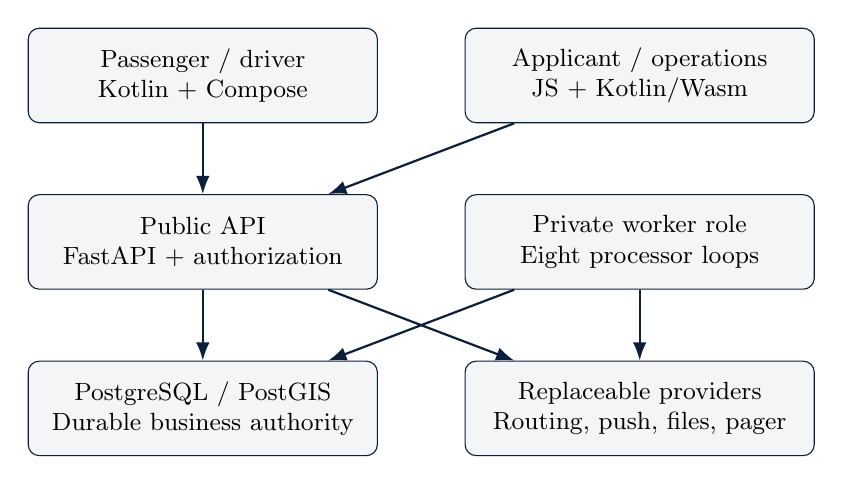
\begin{tikzpicture}[node distance=9mm and 11mm,
box/.style={draw=Navy,rounded corners,fill=Pale,align=center,text width=42mm,minimum height=12mm,font=\small},
arr/.style={-{Latex},thick,draw=Navy}]
\node[box] (mobile) {Passenger / driver\\Kotlin + Compose};
\node[box,right=of mobile] (web) {Applicant / operations\\JS + Kotlin/Wasm};
\node[box,below=of mobile] (api) {Public API\\FastAPI + authorization};
\node[box,right=of api] (worker) {Private worker role\\Eight processor loops};
\node[box,below=of api] (db) {PostgreSQL / PostGIS\\Durable business authority};
\node[box,right=of db] (providers) {Replaceable providers\\Routing, push, files, pager};
\draw[arr] (mobile)--(api);
\draw[arr] (web)--(api);
\draw[arr] (api)--(db);
\draw[arr] (worker)--(db);
\draw[arr] (api)--(providers);
\draw[arr] (worker)--(providers);
\end{tikzpicture}
\end{center}

The public API and worker are separate process roles from the same backend
image. SQLAlchemy/asyncpg provide asynchronous persistence; Alembic governs
migration history; PostGIS supplies geographic predicates. Neither a mobile
cache, the browser, push payload nor a routing response can assign a driver or
confirm payment. PostgreSQL remains authoritative across API replicas.

The initial design deliberately does not require Redis or an external task
queue. A transactional outbox and PostgreSQL live-event fanout provide the
existing asynchronous boundary. Additional infrastructure must be justified by
measurements rather than introduced to make the diagram appear more distributed.
The topology shown is source/deployment design, not evidence of running hosts.

\subsection{Module organization}
\begin{lstlisting}
TaxiMobile/  shared Kotlin, Android flavors, iOS schemes, web roots
backend/     API domains, integrations, workers, migrations, tests
infra/       local stack, deployment blueprints, validation and recovery
assets/      source graphics, exports and reproducible asset tooling
docs/        normative contracts, evidence, workflow and communication
\end{lstlisting}
Shared client code separates data gateways and DTOs, domain contracts, feature
coordinators, UI components and native adapters. The browser has independent
applicant and operations composition roots; it is not a browser port of the
passenger ride UI. Desktop/JVM is useful for development and UI tests, but is not
proof of Android or iOS runtime behavior.
\evidence{\src{backend/src/taximobile_api/api/v1/router.py}, \src{workers/application.py} under the backend package, and \src{TaxiMobile/shared/src/}.}

\section{HTTP contracts and command semantics}
The versioned HTTP surface is rooted at \src{/api/v1}. FastAPI router mounting and
OpenAPI expose the implemented contract. The narrative API document defines
intended conventions and policy, but a prose inventory must not be mistaken for
a callable route. Current source validators expand 82 mobile HTTP operations,
one mobile WebSocket operation and 98 web HTTP operations against backend paths.
This detects method/path drift, not every payload or authorization defect.

\subsection{Command processing sequence}
For a state-changing command, the implementation must establish authenticated
identity and current server session, check ownership or scoped permissions,
validate request shape, load the relevant authoritative records, apply required
locks and fresh eligibility checks, then persist state and associated durable
effects. Response handling must retain the distinction between a rejection and
an unknown outcome after a network failure.

Idempotency protects a documented command scope with a stable key and request
identity. It does not mean that arbitrary requests can be replayed with new keys.
For example, a lost response after cash settlement must be resolved by the same
documented idempotency contract or an authoritative receipt read, not by presenting
another collection operation as a new financial event.

\subsection{Error and recovery behavior}
The client retains backend-confirmed state under the localized offline warning
when usable state exists. Initial failure without usable state uses the dedicated
retry surface. Connectivity restoration prompts a read; it does not acknowledge
a command. Competing actions are gated while a mutation is active, with release
of the gate even on failure. Foreground recovery and push hints also restore
authoritative state without automatically repeating ride or payment commands.
\gate{Contract negative tests, actual browser journeys, physical network-loss
tests, version compatibility and host/CORS/CSP acceptance remain distinct gates.}

\section{Identity, sessions and operations authorization}
Passwords are verified through Argon2; login reduces the dominant absent-account
timing shortcut by performing a verification for active, suspended and absent
identifiers. JWT validation is constrained by issuer, audience, token type and
lifecycle claims, with current server session/account status checked beyond the
token signature. A previously issued token is not sufficient authority after
account suspension or session revocation.

Mobile access and refresh sessions are separate from operations sessions.
Operations authority adds active scoped grants, MFA, recent-MFA requirements and
secure-cookie/CSRF behavior. Scope is a server-side authorization condition,
not merely a browser filter. The legacy administrator router family is mounted
conditionally; its development/compatibility existence must not be generalized
into production global authority.

\subsection{Recovery and remaining lifecycle work}
The mobile offline-code path creates eight independent 100-bit codes after
current-password reauthentication. Domain-separated digests are stored; the
one-time plaintext bundle is shown only for user custody. The documented code
expiry is 180 days. Successful recovery consumes the set under locks, changes
the password and revokes mobile/operations sessions and push registrations in
one transaction. Staff identities cannot use this ordinary mobile recovery path.

Current source includes saved-code acknowledgement, account-owned session lists,
confirmed revocation and password change. Verified email/phone ownership,
delivery-based reset, self-service deletion and personal-data export remain
missing. Offline codes cannot be advertised as verified-contact recovery.

The staff-access UI now supports reviewed create/revoke commands, typed
confirmation, scope selection and non-replay after MFA. It is no longer accurate
to call it read-only. Independent approval, an authoritative staff lifecycle and
last-admin continuity remain open governance/software work.
\evidence{\src{domains/auth/}, \src{domains/administration/}, shared account/auth features and web staff-access modules; paths under \src{backend/src/taximobile_api/} unless qualified.}
\gate{GAP-005, GAP-020, GAP-021 and GAP-022 require policy, physical secure-save,
staff enrollment, recovery and independent-approval evidence.}

\section{Ride aggregate, offers and state transitions}
The persistent live ride states are shown below. Offers have their own
\src{PENDING}, \src{ACCEPTED}, \src{DECLINED}, \src{EXPIRED} and \src{CANCELLED}
states. In particular, ``offered'' is not an additional value in the current
\src{RideStatus} enum; diagrams must not conflate offer state with ride state.

\begin{lstlisting}
REQUESTED -> MATCHING -> ACCEPTED -> DRIVER_EN_ROUTE
          -> DRIVER_ARRIVED -> IN_PROGRESS -> COMPLETED

REQUESTED / MATCHING may terminate without assignment as UNMATCHED.
Permitted pre-trip cancellation paths terminate as CANCELLED.
Offers are separate records with independent expiry/acceptance state.
\end{lstlisting}
The first two lines represent the successful sequence, not a direct jump from
\src{REQUESTED} to arrival. A passenger can cancel the documented pre-trip
states; a driver can cancel only the assigned states before the trip begins.
In-progress exception handling requires its documented safety/operations path
and must not erase the active history through ordinary cancellation.

Ride creation snapshots applicable city/operator/service and financial context.
Acceptance establishes an authorized participant relationship. Completion
finalizes the fare and creates a pending payment; it does not assert collection.
Participant reads constrain access by ownership and lifecycle, including the
limited post-assignment driver visibility.
\evidence{\src{domains/rides/models.py}, \src{domains/rides/service.py}, \src{tests/unit/test_ride_state_machine.py} and \src{tests/integration/test_mvp_lifecycle.py} under \src{backend/}.}

\section{Dispatch eligibility, ranking and contention}
Matching is server-side and deterministic. Candidate discovery checks active
driver and user state, verification, vehicle status, city/service authorization,
credentials, availability, fresh location, geographic radius and competing ride
or protected scheduling commitments. The geographic candidate set is bounded
before ranking. Ranking uses proximity, idle time and recent assignment signals
under a versioned policy; this report does not invent new weights or a new
dispatch objective.

The implementation separates discovery from ownership. Discovery does not lock
every nearby candidate. The service locks a selected driver with
\src{FOR UPDATE ... SKIP LOCKED}, checks current global account authority and
revalidates eligibility using a fresh statement snapshot. If a discovered
candidate is locked or changed, another ranked candidate may be tried. Temporary
contention must not be reported as true absence of supply; bounded worker retry
and the overall matching deadline resolve the still-matching request.

\subsection{Database invariant}
Let $A=\{\text{ACCEPTED},\text{DRIVER\_EN\_ROUTE},
\text{DRIVER\_ARRIVED},\text{IN\_PROGRESS}\}$. The schema enforces:
\[
 \forall d,\quad \left|\{r:r.driver\_id=d\land r.status\in A\}\right|\leq 1.
\]
Migration 0048 creates a partial unique index over assigned drivers in these
states. Before creation it locks ride writes and checks for pre-existing
conflicts; it refuses the migration rather than rewriting ride history. Service
locks protect the command protocol, while the database invariant also constrains
bypassing writes and mixed immediate/scheduled origins.

\evidence{\src{domains/matching/service.py}, \src{domains/matching/scoring.py},
\src{migrations/versions/20260903_0048_one_active_ride_per_driver.py}, and assignment,
live-command, scheduling and dispatch-contention integration tests.}
\gate{Local two-session races support correctness but do not establish fairness
or latency under actual city traffic, API replica count and sparse supply.}

\section{Fixed routes and scheduled handoff}
A fixed route is a versioned published direction with start, finish, optional
stops, static geometry and an explicit flat transport fare. Direction publication
is a configuration workflow, separate from current driver availability. The
catalog must remain truthful when no vehicle is online. Driver acceptance still
uses eligibility and service authorization.

A scheduled booking is a separate aggregate until live dispatch handoff. Its
policy records booking horizon, offering/opening windows, cancellation terms and
surcharge. A future driver commitment does not create an active live ride early.
Acceptance and handoff recheck availability, credential/account authority,
location and protected commitments at their relevant decision boundaries.

Handoff must either establish the consistent live-ride relationship or roll back
and take the documented fallback/unfulfilled path. Retrying after a transaction
failure must not create multiple live rides. The integration suite includes
scheduled acceptance, location/authority races, live protection and handoff
rollback/replay cases. Those are software evidence; real punctuality and passenger
comprehension require field acceptance.
\gate{Approve city route geometry and operating policy, test physical navigation,
and measure scheduled fulfillment before enabling the service for real users.}

\section{Financial model and exact arithmetic}
Pricing is independent of ranking. The backend calculates monetary values with
\src{Decimal}, rounds with \src{ROUND_HALF_UP} to \src{0.01}, and validates currency,
policy shape, fee base and the configured driver-net floor. Clients display
returned amounts and never reconstruct authoritative money from floating point.

Let $T$ be transport fare, $S$ the scheduling surcharge, $F$ the operator service
fee, $S_d$ the portion of the surcharge allocated to the driver and $S_o$ the
portion allocated to the operator. The current closed beneficiary policy gives
$S_d+S_o=S$. Let $a=1$ when the fee is a passenger surcharge and $a=0$ when it is a
driver settlement deduction. Within the validated, rounded policy:
\begin{align*}
 F &= \operatorname{round}_{0.01}(T\,p/100)\quad\text{or an explicit flat fee},\\
 P &= T+S+aF,\\
 D &= T+S_d-(1-a)F,\\
 O &= F+S_o,\\
 P &= D+O.
\end{align*}
$P$ is passenger total, $D$ driver net and $O$ operator allocation. This
conservation identity describes a financial snapshot, not a bank payout.
Immediate rides have no scheduling policy and $S=0$. Percentage mode requires
the documented transport-fare base and a rate below 100; invalid combinations
or a violated driver floor are rejected.

For an illustrative, non-approved tariff with $T=100.00$, $S=0$ and $F=10.00$:
a driver deduction yields $(P,D,O)=(100,90,10)$; a passenger surcharge yields
$(110,100,10)$. These are arithmetic examples only, not Moroccan fare policy.
Version IDs, funding mode, beneficiary and component amounts are preserved in
quote, ride, payment and earning provenance. Later configuration changes must
not retroactively change accepted instructions or historical amounts.
\evidence{\src{domains/pricing/service.py::calculate_financial_quote},
\src{domains/payments/service.py::create_driver_earning}, city economics and cash-workload tests.}

\section{Cash, transfer claims, refunds and the payout gap}
\subsection{Separate service and payment lifecycles}
Completion of a journey creates a pending payment. In cash service, an authorized
driver confirms receipt through the payment command. For manual transfer,
the passenger submits a claim using backend-issued instructions; processing
means awaiting reconciliation, not paid. An authorized scoped reviewer locates
external evidence and verifies or rejects the claim. UI confirmation by the
passenger is never payment authority.

For non-legacy cities, capabilities resolve the exact active service bundle,
operator assignment and effective payment-capability version. Transfer recipients
and instructions are snapshotted. Deployment-global recipient fallback is
legacy compatibility, not a national configuration strategy. Cash remains
first-class; reserved provider enum values are not advertised capabilities.

\subsection{Refund invariants}
Confirmed refunds are append-only records linked to a completed payment. The
command uses payment locking, positive exact amounts, evidence, a closed reason
taxonomy, audit and idempotency. Cumulative refunds cannot exceed the completed
amount. The implemented launch policy assigns full operator funding and zero
driver recovery. It does not permit silently raising a completed fare or
rewriting historical earnings.

\subsection{Missing settlement accounting}
Driver earnings are not a complete operator-to-driver ledger. GAP-024 identifies
missing settlement periods, payable balances, cash offsets, payout instructions,
remittance statements, reconciliation and correction policy. These need an
approved accounting model before new schema or payout behavior is introduced.
Card/CMI remains deferred and is not a substitute for completing the launch
cash/manual-transfer operating model.
\gate{Controlled recipient verification, exact statement matching, cash custody,
refund execution, reconciliation staffing and accountant-reviewed payout examples.}

\section{Outbox, live hints and background execution}
Durable business events are recorded with state changes so notification delivery
can be retried without inventing business success. PostgreSQL fans minimized
refresh hints across API instances. Connected clients use authenticated live
events; background devices use the FCM/APNs boundary and then reload authorized
resources. A delivered hint is not a payment receipt, and a missing hint is not
proof that a transaction failed.

Outbox processing contains bounded retry, ownership/lease handling, dead-letter
state and reviewed replay. Invalid registrations can be revoked. Event payloads
and metrics must not expose exact locations, payment instructions or safety text.
Provider outages must retain observable backlog and actionable operational
signals, rather than reporting a false healthy count.

\begin{table}[H]\centering
\begin{tabular}{@{}p{.24\textwidth}p{.69\textwidth}@{}}
\toprule Worker loop & Responsibility \\\midrule
Matching & Advance pending dispatch and offer expiry/retry. \\
Outbox & Deliver durable events and handle retries/dead letters. \\
Credentials & Apply credential lifecycle effects to eligibility. \\
Scheduling & Advance due bookings, offering and dispatch handoff. \\
Analytics & Refresh bounded aggregate projections. \\
Case alerts & Route overdue support/safety escalation and acknowledgement. \\
Case retention & Apply eligible minimization while respecting legal holds. \\
Driver-document retention & Retire eligible protected document data through the configured store. \\
\bottomrule
\end{tabular}
\end{table}
The supervisor owns task lifecycle and deterministic cancellation, not business
concurrency authority. Database locks and leases remain authoritative. Worker
readiness requires the supervisor and positive progress from all eight loops;
process liveness alone does not establish useful processing.

\section{Maps, place discovery and foreground location}
MapLibre composes maps on the native platforms. The backend normalizes selected
Valhalla or GraphHopper routing behind a shared route contract. The geocoding
boundary offers authenticated search/reverse lookup with a fail-closed
Nominatim-compatible adapter and PostGIS service-area authority. Search results
are not themselves permission to request a pickup outside an enabled boundary.

The client can retain useful route/point overlays when map styling fails, with a
documented neutral fallback. Source includes one-shot current-location admission
and a foreground-only online driver heartbeat. Describing the driver experience
as only one-shot is stale; describing it as continuous background tracking is
also incorrect. Stale/unavailable location can reduce eligibility, so device
permissions, battery, foreground behavior and weak networks are operational
dispatch requirements rather than cosmetic map tests.

English, French and Arabic UI catalogs do not establish equivalent routing
narration. The documented pinned Valhalla catalog lacks accepted Arabic spoken
guidance. The existing routing acceptance runner deliberately refuses to count
an English fallback as Arabic success. A real graph, data/license review,
multilingual place benchmark and device navigation matrix remain open.
\gate{GAP-006--009 and GAP-026: graph/style/geocoder acceptance, query privacy,
foreground location quality, narration and real background notification delivery.}

\section{Client state, localization and release boundaries}
Passenger and driver are separate Android flavors and iOS targets/schemes over
shared Kotlin. Shared coordinators and gateways enforce common presentation
behavior; native source sets implement secure token storage, connectivity,
current location, MapLibre integration and notification receive paths. Reuse
does not eliminate native testing: background execution, permissions, keychain
behavior, accessibility and app lifecycle differ by platform.

The approved interface is map-first with role-specific actions and an explicit
mustard/navy/white identity. Loading, empty, error, offline, unavailable and
permission-denied states are part of the product contract. A success animation
requires backend-confirmed success. Localization has English/French/Arabic
catalogs and RTL treatment, but translation parity cannot prove reading order,
clipping, assistive technology or low-literacy usability.

Android release source includes role separation and configuration checks. iOS
simulator compiler gates require macOS; Windows JVM success does not execute
iOS. Signed artifacts, provider-specific release configuration, R8/dSYM handling,
controlled Crashlytics reports and store acceptance remain separate evidence.
Browser component tests exercise JS/Wasm code; end-to-end applicant, protected
document and staff journeys still require the actual hosted security model.

\section{National control plane and configuration consistency}
The control plane models markets, operators, city assignments, service areas,
service configuration and scoped staff authority. Tariffs, scheduling rules,
operator fees, payment capabilities and fixed-route publication are versioned.
A coherent city bundle resolves compatible reviewed references; the browser
must not manufacture authoritative configuration by concatenating arbitrary JSON.

The product lifecycle progresses through draft/configuration and controlled
pilot/active states, with emergency pause and post-launch review. The backend can
validate record shape, reference consistency, permissions and recorded evidence.
It cannot determine that an uploaded legal document is valid or that the duty
roster will answer a real incident. Source readiness controls are mechanisms
for governance, not independent proof of operational readiness.

Sensitive staff mutations now have create/revoke UI and recent-MFA checks.
However, one authorized administrator can still perform actions that may need
independent approval. Scope isolation and self-action protection are not the same
as dual control. GAP-022 leaves the maker/approver policy and last-admin continuity
unresolved; this report does not introduce a new approval state machine.

\section{Protected documents, safety and privacy lifecycle}
Driver applications have a special protected PDF/JPEG/PNG workflow, not a general
file-upload permission. Storage and malware scanning must be configured; adapters
fail closed when prerequisites are missing. Access follows applicant/authorized
reviewer scope, while encryption, retention and document-access evidence require
production operation of the selected store/scanner/key boundary.

Support and safety are separate records with distinct visibility. Operations
queues, assignment, notes, status transitions, minimal safety handoff, overdue
paging and acknowledgements exist. Restricted narratives must not leak into
ordinary support views, broad audit fields or push payloads. Legal holds and
retention workers constrain eligible minimization; erased material must not be
returned by read endpoints.

The platform is not an emergency-dispatch service. A safety report must explain
its limitations and the approved local emergency direction. Real staffing,
escalation, on-call coverage and incident drills remain necessary even when every
case API test passes. Account deletion/export and cross-store privacy-right
handling remain incomplete. Database erasure alone cannot demonstrate expiry in
backups, logs, document stores and third-party systems.
\gate{GAP-011/012/017/021/030/031: accepted legal basis, retention policy,
cross-store evidence, document safety, staffed response and security incident operations.}

\section{Deployment, migrations, monitoring and recovery}
Production manifests separate public API and private worker roles, restrict
operations surfaces and apply readiness checks. Monitoring includes bounded
JSON logs, authenticated metrics and hardened Prometheus/Alertmanager/Loki/Alloy/
Grafana definitions. Fixed-name loop progress, outbox pending/dead-letter state
and snapshot availability provide observable failure indicators without exposing
participant data as labels.

These files are blueprints and validators. They do not establish deployed TLS,
private database networking, managed secrets, image registry provenance, paging
ownership, log-store availability or accepted operating cost. Host selection and
deployment remain owner decisions. No infrastructure was provisioned by this audit.

\subsection{Migration and disaster recovery}
The current Alembic chain has 48 migrations through \src{20260903_0048}. A release
requires a current-head upgrade rehearsal, meaningful integrity checks and
application readiness against the target environment. Offline SQL rendering is
useful review material but cannot prove a live migration succeeds under locks,
permissions, historical data and deployment timeouts.

Existing documentation records an older backup/restore drill at migration 0029.
It remains historical evidence and must not be relabeled as a 0048 restore.
Production acceptance needs an isolated restore, measured recovery time,
approved RPO/RTO, encryption and backup-expiry/legal-hold reconciliation. A
forward-fix or rollback decision must account for schema compatibility and
irreversible data changes; blindly running downgrade is not a universal recovery
procedure.

\section{Verification performed and evidence limits}
For this documentation assessment, backend unit/API verification passed
\textbf{699 tests} with 173 dependency deprecation warnings in 45.52 seconds.
The infrastructure script suite passed 11 tests; the mobile script suite passed
30. Mobile/backend and web/backend source contract checks passed 82 HTTP plus
one WebSocket operation and 98 HTTP operations respectively.

The shared JVM suite was then forced to execute with \src{--rerun-tasks --offline}:
\textbf{178 tests passed}, with zero failures, errors or skips. Final documentation
and PDF checks are recorded in \src{docs/readiness.md}. No fresh PostGIS database
rebuild was run for this documentation-only assessment. Existing project records
report 819 full backend tests on fresh PostGIS, 178 shared JVM tests and Android/
JS/Wasm verification. Those database/platform results remain historical claims
unless explicitly rerun in the assessment table.

The current CI definition includes backend/PostGIS, Android/shared, iOS simulator,
web JS/Wasm and documentation/provenance checks, plus supply-chain controls. Its
presence in a dirty working tree is not a passing remote run, complete SBOM
acceptance, signed artifact or independent vulnerability assessment.

\subsection{Test-layer interpretation}
\begin{tabularx}{\textwidth}{@{}p{.19\textwidth}XX@{}}
\toprule Layer & What it can establish & What it cannot establish alone \\\midrule
Unit/API & Policy branches, decoding, validation and isolated route behavior & Real row locking, native delivery or production availability. \\
PostGIS integration & Schema behavior, transactions, races and persisted lifecycles & City-scale traffic or accepted providers. \\
JVM/browser components & Shared coordinator/UI and browser model behavior & Physical device or complete hosted journey acceptance. \\
Staging and load & Measured behavior for a specified candidate and workload & Legal authority, adoption or unspecified capacity. \\
Staff/field/pilot & Operational readiness within the approved bounded scenario & Unlimited national scale or future policy correctness. \\
\bottomrule
\end{tabularx}

\clearpage
\section{Weighted implementation matrix}\label{sec:score}
The rating scale is 0: requirement only; 1: scaffold; 2: material implementation
with a major missing workflow; 3: main path/tests with meaningful remaining
source or integration scope; 4: defined core source path and meaningful tests
across its boundaries. Four is not deployment acceptance. Weights are explicit
assessment judgments and sum to 100, partitioning engineering scope rather than
counting files or completed roadmap phases.
\[
 C=\sum_i w_i\frac{s_i}{4}=\frac{336}{4}=84\%.
\]
\begin{table}[H]\centering
\begin{tabular}{@{}p{.55\textwidth}rrr@{}}
\toprule Workstream & Weight & Rating & Points \\\midrule
Identity and recovery & 8 & 3 & 6.00 \\
Driver recruitment and eligibility & 8 & 4 & 8.00 \\
Immediate rides and coordination & 10 & 4 & 10.00 \\
Matching and assignment integrity & 8 & 4 & 8.00 \\
Pricing and immutable economics & 7 & 4 & 7.00 \\
Payments and settlement & 8 & 3 & 6.00 \\
Fixed routes and scheduling & 7 & 4 & 7.00 \\
Passenger/driver mobile & 10 & 3 & 7.50 \\
Applicant/operations web & 7 & 3 & 5.25 \\
Maps, places, navigation and delivery & 6 & 3 & 4.50 \\
Support and safety & 5 & 3 & 3.75 \\
City control plane and governance & 5 & 3 & 3.75 \\
Privacy rights and data lifecycle & 4 & 2 & 2.00 \\
Analytics & 2 & 3 & 1.50 \\
Deployment and observability tooling & 3 & 3 & 2.25 \\
CI, supply chain and release tooling & 2 & 3 & 1.50 \\\midrule
\textbf{Total} & \textbf{100} & & \textbf{84.00} \\\bottomrule
\end{tabular}
\end{table}
The companion Markdown matrix links each row to implementation and remaining
GAP IDs. Missing payout/account lifecycle/dual-control paths keep their rows
below four even when individual modules are mature. Additional tests or source
files do not automatically increase a rating. Reassess when scoped behavior or
its evidence changes. P0 closure remains a separate veto: 0/19 accepted, not a
claim that no engineering work exists.

\section{Documentation reconciliation}
The audit corrects forward-looking migration references from 0046 to 0048 in
the documentation index and database-rehearsal gap. Historical 0046 and older
restore/test results retain their original dates and heads. The TeX artifacts
are rewritten because their browser, staff-access and location descriptions
lagged behind the implementation.

The extended UI introduction now refers to service discovery and authorized
post-assignment tracking, consistent with existing supply privacy. This resolves
misleading wording rather than approving pre-assignment driver browsing. The
client README still contains stale text about MFA/cookie/CSRF not being
implemented; that non-\src{docs/} discrepancy is recorded for a focused follow-up.
No architecture or business policy was changed to fit implementation convenience.

\section{Delivery workflow and acceptance ownership}
The new \src{docs/workflow.md} provides the practical sequence. Start from the
dated assessment and relevant GAP, then read the owning domain, roadmap and
affected API/database/security/UI contracts. Inspect existing code before adding
a duplicate path. Define the actor, scope, trigger, permitted state change,
rejected cases and evidence boundary before implementation.

Deliver one complete behavior slice: backend authority and transaction, necessary
schema/API change, shared gateway/coordinator, native integration, honest UI and
meaningful negative/failure tests. Update the owning documentation. A conflict
with a normative rule pauses the affected implementation until the owner resolves
it; it does not justify silently editing policy.

\begin{enumerate}
\item T0--T2: static/source contracts, unit/component tests and simulated personas.
\item T3: isolated migrated PostGIS and complete multi-role local lifecycles.
\item T4: browser, emulator and physical-device lab with language and failure cases.
\item T5: identified candidate in production-like staging, including restore,
providers, performance and security.
\item T6: trained staff rehearse synthetic cases, money controls, paging and recovery.
\item T7: explicitly bounded non-public field validation under approved safeguards.
\item T8: authorized real-user pilot only after applicable P0 evidence closes.
\item T9--T10: public-city acceptance, monitoring, closeout and repeatable expansion.
\end{enumerate}

Every handoff records candidate commit/tree, artifacts, schema head, environment,
city/provider versions, scenario IDs, observed result, evidence location and
owner/reviewer decision. Changed source/configuration may invalidate evidence.
A job marked CI-wired is not an intermediate proof of successful execution.

\section{Priority work and decision dependencies}
\begin{table}[H]\centering
\begin{tabular}{@{}p{.15\textwidth}p{.42\textwidth}p{.35\textwidth}@{}}
\toprule Sequence & Work package & Exit evidence \\\midrule
1 & Review dirty source, untracked migrations/assets and candidate completeness & Clean candidate, complete remote CI, artifact hashes and reviewed provenance. \\
2 & Resolve verified identity, privacy rights, dual control, payout and retention policy & Domain decisions, implementation tasks and negative/integration acceptance. \\
3 & Establish isolated hosted staging and selected providers & Current-head restore, controlled maps/push/files/money and monitoring evidence. \\
4 & Finish device/browser/security/capacity gates & Signed candidate matrix, independent review, defined load and failure results. \\
5 & Establish accountable city and operating organization & Legal/operator evidence, trained roster, safety/payment/incident drills and stop criteria. \\
6 & Promote through bounded field and pilot gates & Explicit owner approval and measured outcomes before public activation or expansion. \\
\bottomrule
\end{tabular}
\end{table}
Policy-dependent software work cannot be completed by an audit estimate. Named
owners, tariff rules, legal structure, settlement accounting and deployment
choices remain decisions for the project owner and accountable operators.
The assessment supplies a reviewable order and evidence requirements, not an
invented schedule or budget.

\appendix
\clearpage
\section{Source and requirement traceability}
Paths in the following table are relative to the repository root. Domain code
directories referenced earlier are under \src{backend/src/taximobile_api/}.
\begin{table}[H]\centering
\begin{tabular}{@{}p{.25\textwidth}p{.67\textwidth}@{}}
\toprule Subject & Primary repository references \\\midrule
Product and authority & \src{docs/product.md}, \src{docs/architecture.md}, \src{AGENTS.md} \\
Contracts and state & \src{docs/api.md}, \src{docs/database.md}, \src{docs/rides.md}, \src{docs/matching.md} \\
Economics & \src{docs/pricing.md}, \src{docs/payments.md}, pricing/payment services and cash workload tests \\
Identity and governance & \src{docs/auth.md}, \src{docs/operations.md}, administration/auth domains and operations web \\
Privacy and safety & \src{docs/security.md}, \src{docs/threat_model.md}, support/safety/retention domains \\
Client behavior & \src{docs/design.md}, \src{docs/ui.md}, \src{docs/extended_ui.md}, shared/native/web client source sets \\
Test evidence & \src{docs/testing.md}, \src{docs/testing_workloads.md}, backend/client tests and source validators \\
Delivery and assessment & \src{docs/workflow.md}, \src{docs/readiness.md}, \src{docs/gaps.md}, \src{docs/roadmap.md} \\
Runtime/release & \src{infra/deploy/}, \src{infra/scripts/}, \src{.github/workflows/ci.yml} \\
\bottomrule
\end{tabular}
\end{table}

\section{Reproduction and publication notes}
Use the executable commands in \src{docs/workflow.md}. The guarded portable
backend runner rebuilds the isolated \src{taximobile_ci} database and must be
coordinated with other local test users. Do not use a production database for
integration fixtures. Do not print local environment credentials to manufacture
an evidence report.

Compile this document and the technical briefing twice with pdfLaTeX, inspect
logs and rendered pages, then retain matching TeX/PDF versions. Local PDF build
success certifies document syntax/layout only, not the implementation claims.
The current readiness table identifies which software checks were actually
rerun. All percentages, examples and historical results must retain their scope
when excerpts are reused in presentations or project discussions.
\end{document}
